\section{Signed residuals and strong versions of the old shortcut}
\label{sec:signed-experiments}

The additional benefit here is the ability to use negative residuals directly.
For a fitted base interval $[\ell_j(x),u_j(x)]$, write its midpoint as $m_j(x)$
and half-width as $h_j(x)$. The signed quantile residual is
\[
 r_j(x,y)=\max\{\ell_j(x)-y_j,\,y_j-u_j(x)\}
         =|y_j-m_j(x)|-h_j(x)\geq-h_j(x).
\]
A negative threshold contracts the fitted interval. The envelope uses these
raw scores and the attainable candidate domain $[-h_j(x),\infty)$ directly.
The old shortcut's nonnegative-score construction requires a transformation;
we give it three valid versions, all fixed by the training fit:
\begin{enumerate}
\item \emph{Capping}: use $r_j^+=\max(r_j,0)$. This discards the depth of
  observations inside the base interval and cannot contract the base.
\item \emph{Constant shift}: set $c_j=\max_{g\in\{0,1\}}h_{gj}$ and use
  $r_j+c_j$. This is the smallest constant coordinatewise shift certified by
  the fitted base widths over both covariate groups. Subtract $c_j$ from the
  old threshold when mapping back to the outcome space.
\item \emph{Width shift}: use $r_j(x,y)+h_j(x)=|y_j-m_j(x)|$. Subtract
  $h_j(x)$ from the old threshold at prediction. This is a covariate-dependent
  transformation, rather than a common translation, and is also nonnegative
  for every future observation.
\end{enumerate}
Both shifts preserve the residual value when their known offsets are retained;
neither uses a calibration minimum. In particular, signed support is an
advantage of the new construction, but does not mean the old method has no
valid workaround. No envelope calculation is applied to capped residuals in
these comparisons.

We use three settings, each with 120 paired fitted trials, 800 training
observations, $n=80$ calibration observations, 1,200 test observations and
$\alpha=0.1$. Two settings have Gaussian noise and two outcomes, with fitted
nominal marginal base coverage levels of 90\% and 98\%; the wider base deliberately
tests contraction. The third has Laplace noise and six outcomes with a 90\%
marginal base. The data model and OLS training procedure are the same as in the
absolute-residual experiments. To fit the base intervals, compute training
errors $Y_j-\widehat f_j(X)$ separately in the two groups $g(X)=0,1$.
If $\delta$ is the base miscoverage (0.1 or 0.02), let $a_{gj}^-$ and
$a_{gj}^+$ be their empirical $\delta/2$ and $1-\delta/2$ quantiles.
Then $\ell_j(x)=\widehat f_j(x)+a_{g(x),j}^-$ and
$u_j(x)=\widehat f_j(x)+a_{g(x),j}^+$. These offsets are estimated only
from training data; nominal base coverage need not equal achieved joint
coverage. All four methods receive the same observations
and fitted intervals within a trial. We compare every version separately;
identifying the smallest average old volume below is a descriptive comparison,
not a rule that chooses a method on calibration or test outcomes.
These 360 trials reuse the prior fitted observations; the shifted baselines
are newly evaluated in this revision. The 120 six-output Laplace fits also
appear in the absolute study, so the two sections are paired views of those
fits, not independent additional evidence. For a threshold $L_j(x)$, the
outcome volume is $\prod_j\{2h_j(x)+2L_j(x)\}$ when all coordinate lengths
are nonnegative, and zero if any coordinate interval is empty. Each trial
averages this volume over its 1,200 test inputs before paired ratios are
formed; zero-length singleton intervals have zero volume but are retained.

\begin{figure}[tbp]
\centering

\includegraphics[width=\linewidth]{figures/signed_comparison.pdf}
\caption{Raw signed envelope versus three valid nonnegative versions of the
old shortcut. Top: simultaneous test coverage. Bottom: mean paired outcome
volume ratios, with the named old version as denominator. Bars are pointwise
95\% Monte Carlo intervals across independent fitted trials. All coverage
summaries include infinite regions. Only the wide-base capped comparison
excludes nonfinite volume pairs: 91 of 120 pairs remain; the other 29 capped
regions are infinite. Every other ratio uses all 120 pairs.}
\label{fig:signed-comparison}
\end{figure}

Figure~\ref{fig:signed-comparison} shows why the shifted baselines matter.
With the ordinary 90\% Gaussian base, capping has the smallest average old
volume; the envelope's mean paired volume is $0.42\%$ larger, with a 95\%
interval of $[-0.23\%,1.07\%]$ for this difference. Thus there is no empirical
gain over the strongest old version in this setting. With the 98\% Gaussian
base, old capping is overconservative (coverage $0.9613$, MCSE $0.0022$) and
produces infinite regions in $29/120$ trials under the stated zero-scale
fallback: at least one coordinate has all capped calibration scores equal
to zero. This is a conservative implementation convention, rather than a
claim that every possible treatment of capped ties must be infinite.
The two shifts remove that
problem. The constant shift has the smallest average old volume, and the
envelope reduces the paired volume by $1.79\%\pm0.12\%$ relative to it;
coverage is $0.9071$ (MCSE $0.0026$), versus $0.9114$ (MCSE $0.0025$) for
the constant shift. Negative envelope adjustments occur in 88.7\% of
test-coordinate cases, illustrating contraction of an overly wide base.

For the six-outcome Laplace setting, the envelope's paired volume reduction
is $15.83\%\pm3.89\%$ relative to old capping, but $1.46\%\pm0.20\%$
relative to the stronger constant shift. Their coverages are $0.9049$
(MCSE $0.0031$) and $0.9057$ (MCSE $0.0031$), respectively. These small but
consistent gains against a strong shifted implementation are the relevant
size comparison. Changing to capped or covariate-shifted scores also changes
the conformal construction, so these experiments do not assert a universal
ordering across those score choices.

\begin{figure}[tbp]
\centering
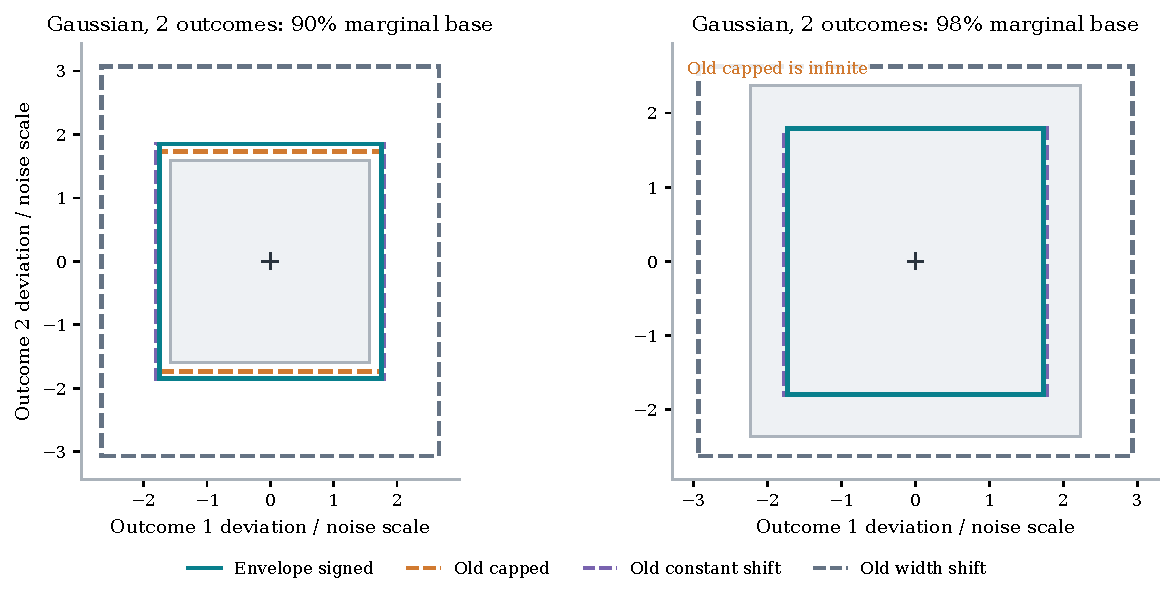
\includegraphics[width=.97\linewidth]{figures/signed_regions.pdf}
\caption{Outcome regions for the two Gaussian settings at predetermined
trial 0 and test observation 0. Axes are deviations from the fitted base
midpoint divided by the coordinate noise scale; the pale rectangle is the
fitted base interval product. The ordinary base need not favor signed
residuals over capping. With the wide base, the signed envelope and the
constant-shifted shortcut both contract it; their size difference is modest.
The width shift is valid but loses the original covariate-dependent base-width
adjustment, which makes its region visibly larger at this observation.
The capped region in the right panel is infinite.}
\label{fig:signed-regions}
\end{figure}
